\documentclass{article}
\usepackage[utf8]{inputenc}
\usepackage{hyperref}
\usepackage[a4paper, total={7in, 8in}]{geometry}
\usepackage{graphicx}
\usepackage{setspace}
\usepackage[left=2.5cm,right=2.5cm,top=3cm,bottom=3cm]{geometry}
\usepackage{array,tabularx,booktabs}
\usepackage{float}
\title{Gruppe31\_Assigment04}
\author{Mathias Fink (matf)\\ Thomas Hoffmann Kilbak(thhk)\\ Oliver Holmberg Jørgensen (ojoe)\\ Group 31}
\date{September 29th 2020}

\begin{document}

\maketitle

\noindent \href{https://github.itu.dk/ojoe/BDSA2020.Assignment04}{Repository for C\# portion of the assignment:} \\
\url{https://github.itu.dk/ojoe/BDSA2020.Assignment04}

\section{Exercise 1}
Consider a file system with a graphical user interface, such as Macintosh’s Finder, Microsoft’s Windows Explorer, or Linux’s KDE. The following objects were identified from a use case describing how to copy a file from a floppy disk to a hard disk: File, Icon, TrashCan, Folder, Disk, Pointer. Specify which are entity objects, which are boundary objects, and which are control (interactor) objects. :\newline
\newline
bruh
File: Entity Object \newline
Icon: Boundary object \newline
Trashcan : Boundary object \newline
Folder : Entity object \newline
Disk : Entity object \newline
Pointer: Boundary object

\section{Exercise 2}
Assuming the same file system as before, consider a scenario consisting of selecting a file on a floppy, dragging it to Folder and releasing the mouse. Identify and define one control (interactor) object associated with this scenario. \newline

The file is copied by the system to allow placing the file in the new destination this would be considered a Control object as it is done by the System due to an action taken by the user. \newline
This control object will be named CopyFile.

\section{Exericse 3}
Arrange the objects listed in Exercises SE.1-2 horizontally on a sequence diagram, the boundary objects to the left, then the control (interactor) object you identified, and finally, the entity objects. Draw the sequence of interactions resulting from dropping the file into a folder. For now, ignore the exceptional cases.

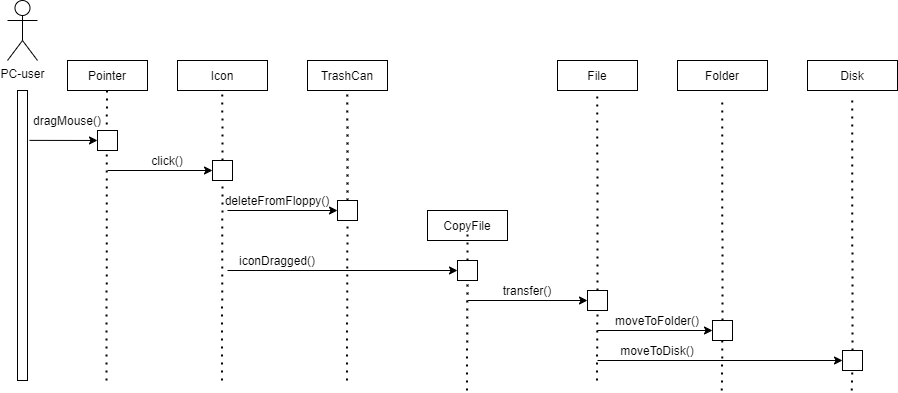
\includegraphics[scale=0.5]{Untitled Diagram.png}


\section{Exercise 4}
From the sequence diagram Figure 2-34, draw the corresponding class diagram. Hint: Start with the participating objects in the sequence diagram.

 
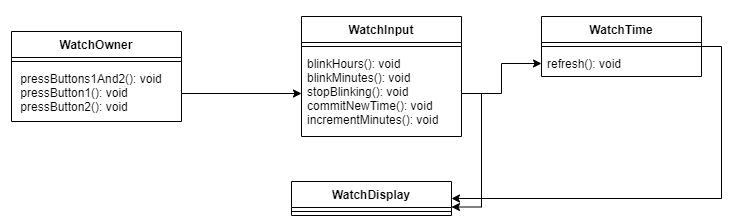
\includegraphics[scale=0.8]{Untitled Diagram (1).png}

\end{document}